%----------------------------------------------------------------------------------------
%	Product description
%----------------------------------------------------------------------------------------
\chapter{Product description} % Main chapter title
\label{Chapter4} % For referencing the chapter elsewhere, use \ref{Chapter4}
This chapter covers the system's design, starting with the complete system architecture and then going into each component in greater detail.


%----------------------------------------------------------------------------------------
%	1. System requirements
%----------------------------------------------------------------------------------------

\section{System requirements}
Initial discovery sessions with the business owners, managers, and receptionists uncovered the requirements for the system and their use cases. These requirements can be split into four types \parencite{cox_business_2021}: business, user, functional and quality.

Business requirements are what the business wants to achieve (Figure~\ref{fig:businessreq}). These are the overall objectives which the project aims to address.

The user requirements are what the user requires the system to provide to achieve the business requirements (Figure~\ref{fig:userreq}). These provide insight into the user stories and support the functional requirements.

Functional requirements describe the software's activities and processes to achieve the user requirements (Figure~\ref{fig:functionalreq}). These are the functions which the system must support that tie into the user requirements.

Quality requirements describe the performance and metrics the functional requirements within the system must achieve(Figure~\ref{fig:qualityreq}).

\begin{table}[ht!]
    \caption{Business requirements}
    \renewcommand{\arraystretch}{1.5}
    \centerline{
        \begin{NiceTabular}{ m{1cm} m{9cm} m{2.5cm}  }
            \hline
            \textbf{ID} & \textbf{Requirement} & \textbf{Priority}\\
            \hline \hline
            BR1 & A system which is accessible within the gym and off-site (residence). The system must be online & Must have\\
            \hline
            BR2 & Multi-device support to view and edit data & Must have\\
            \hline
            BR3 & Unify method of data search and entry & Must have\\
            \hline
            BR4 & Reduce input and search time on data by at least 50\% & Must have\\
            \hline
            BR5 & Increase profit by removing non-payment attendance & Should have\\
            \hline
            BR6 & Provide insights to improve business-making decisions & Should have\\
            \hline
           \end{NiceTabular}
    }
    \label{fig:businessreq}
\end{table}

\ \\

\begin{table}[ht!]
    \caption{User requirements}
    \renewcommand{\arraystretch}{1.5}
    \centerline{
        \begin{NiceTabular}{ m{1cm} m{9cm} m{2.5cm}  }
            \hline
            ID & Requirement & Priority\\
            \hline \hline
            UR1 & Staff must log in to prevent unauthorised access. (Since the system will be available online). The system must be online & Must have\\
            \hline
            UR2 & Staff can input, view and edit member data. (Needed for adding new members and supporting existing customers) & Must have\\
            \hline
            UR3 & Add and edit lessons available for each day. (Lessons must also be tracked for attendance) & Must have\\
            \hline
            UR4 & The receptionist can add members to lessons. (Attendance must be tracked) & Must have\\
            \hline
            UR5 & The receptionist can take payments which correlate to available attendance to lessons. (Lesson type and purchase type length at play) & Must have\\
            \hline
            UR6 & Provide metrics on business performance (member signup, attendance, payment totals) across a date range (day, week, month, year) & Must have\\
            \hline
           \end{NiceTabular}
    }
    \label{fig:userreq}
\end{table}

\ \\

\begin{table}[ht!]
    \caption{Functional requirements}
    \renewcommand{\arraystretch}{1.5}
    \centerline{
        \begin{NiceTabular}{ m{1cm} m{9cm} m{2.5cm}  }
            \hline
            ID & Requirement & Priority\\
            \hline \hline
            FR1 & Add, view and edit members & Must have\\
            \hline
            FR2 & Add, view and edit lessons & Must have\\
            \hline
            FR3 & Add and view payments & Must have\\
            \hline
            FR4 & Add and view purchases & Must have\\
            \hline
            FR5 & Support bulk-purchase of lessons & Must have\\
            \hline
            FR6 & Handle member attendances for lessons based on purchases & Must have\\
            \hline
            FR7 & Provide member, attendance and payment statistics over day, week, month and fiscal year & Should have\\
            \hline
           \end{NiceTabular}
    }
    \label{fig:functionalreq}
\end{table}

\ \\

\begin{table}[ht!]
    \caption{Quality requirements}
    \renewcommand{\arraystretch}{1.5}
    \centerline{
        \begin{NiceTabular}{ m{1cm} m{9cm} m{2.5cm}  }
            \hline
            ID & Requirement & Priority\\
            \hline \hline
            QR1 & Reduce member search time to less than 30 seconds & Must have\\
            \hline
            QR2 & Reduce accounting time by at least half for payments & Should have\\
            \hline
           \end{NiceTabular}
    }
    \label{fig:qualityreq}
\end{table}

\section{Problem solving}
Supporting the user experience while accurately storing the data was lengthy and complex. However, the most complex was solving the issue of lesson bulk-purchase tracking in tandem with attendance.

Were this for single lessons, the purchase could be linked to the attendance making for an outer join solve the problem. However, this would not work since a single purchase could constitute a collection of lessons.

Another solution would be to recalculate upon each attendance request. Each attendance request would count up the total number of lessons remaining by adding up valid payments, deducting past attendances, and finally returning the total number of lessons remaining. This would work, yet it results in longer wait times for receptionists tracking attendance. In addition, as the database grows, the wait time will also grow at an exponential rate.

The solution selected was to create tokens. Lesson purchases will generate tokens allowing access only if tokens are available for the requested lesson. Single lessons generate a token for that type of lesson that lasts seven days (Figure~\ref{fig:single-token}). This solution works similarly to the original idea.

\begin{figure}[ht!]
    \centerline{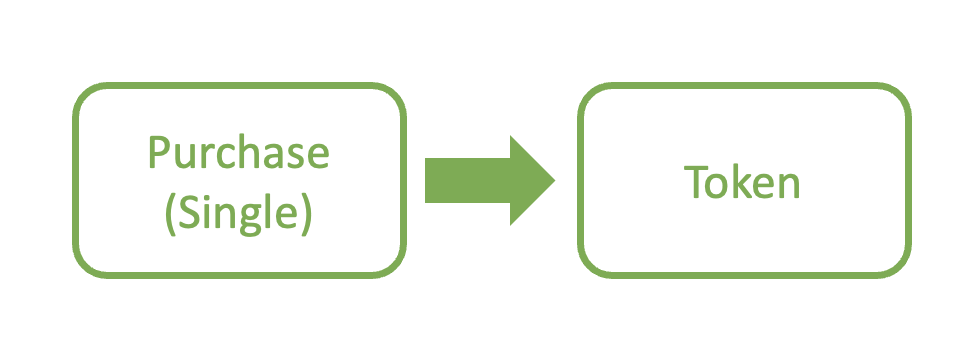
\includegraphics[width=0.5\linewidth]{single-purchase-token.png}}
    \caption{Token generation from single lesson purchase}
    \label{fig:single-token}
\end{figure}

Depending on the lesson type (monthly single, monthly double, etc.), bulk purchases will generate a different quantity of tokens based on the purchase type. This adds a heavier load to when a purchase is made but can be completed quickly since additions are linear, whereas searches are slower when calculating across linked tables.

\begin{figure}[ht!]
    \centerline{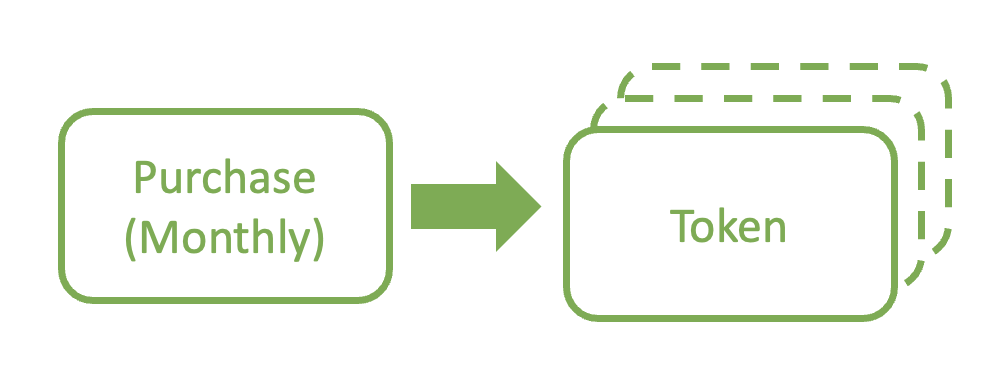
\includegraphics[width=0.5\linewidth]{monthly-purchase-tokens.png}}
    \caption{Multiple tokens generated from monthly lesson purchase}
    \label{fig:multi-token}
\end{figure}

If the member does not have an available valid token, they must either pay now to acquire one for the lesson making for a single lesson purchase or pay later, adding debt to their account.

This solution must be handled within the API and a carefully structured database table to enforce the need for this token for attendance. The correct number and dates must be applied to these tokens to ensure members are not paying and unable to attend due to incorrect validity times. The UI will also need to interact with this, informing the receptionist if the user has a valid token or not.


%----------------------------------------------------------------------------------------
%	2. System architecture
%----------------------------------------------------------------------------------------

\section{System architecture}

\subsection{Software type}
Based on requirement BR1, the data would need to be hosted online in some capacity allowing devices to access a central store of data. For example, this could be through an application or website.

This requirement raised the question of application type. Requirement BR2, which also requires multi-device access, helped narrow the focus to a progressive web application (PWA) \parencite{tandel_impact_2018}.

A desktop application is not portable. Although some languages, such as Java, support running a single compiled binary on many devices, it remains limited to desktop devices. In addition, mobiles and tables would require their native application to be written separately, thus doubling the workload. Likewise, mobile applications would also require a different build for Android and iOS, respectively.

Progressive web applications, and web applications in general, solve this issue. All devices support viewing web application interaction through a browser, and many modern operating systems on desktop and mobile devices support viewing progressive web applications as pseudo-native applications \parencite{biorn-hansen_progressive_2017}. Therefore, these applications can be bookmarked on desktop and mobile devices and behave like native applications.


\subsection{Software structure}
For any application, data storage and system interaction are vital components which must be considered. Combined with the complexity of their pricing and attendance requirements, a logical layer that ties the interaction and the data storage will help separate concerns. This separation creates a 3-tier architecture \parencite{fernandez_secure_2008} which follows the single responsibility, clean code design principle \parencite{martin_clean_2008}.

\begin{figure}[ht!]
    \centerline{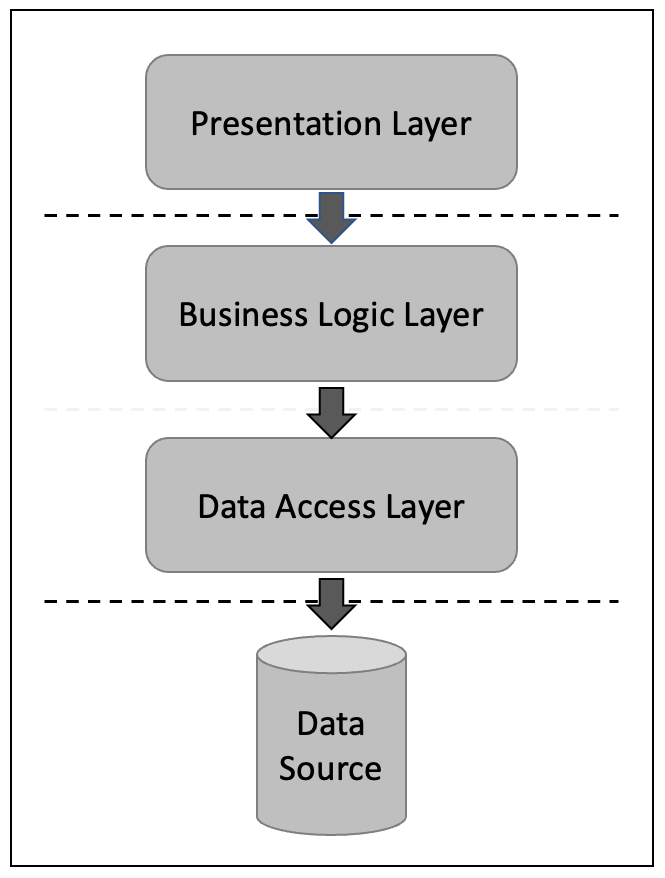
\includegraphics[width=0.5\linewidth]{3-tier.png}}
    \caption{Diagram of the 3-tier system architecture}
    \label{fig:sysarch}
\end{figure}

The three components of this system consist of a data layer, a logic layer and a presentation layer (Figure~\ref{fig:sysarch}). 

The data layer manages data storage and supports data submission, modification, and removal. For this reason, a relational database was selected to handle the storage of member records, attendance and pricing.

The presentation layer expresses the data in a user-friendly manner and handles user input. The display consists of components for displaying the data, such as graphs and elements to add and modify the data, including forms, buttons, text boxes and drop-down menus.

Finally, the logical layer handles the operations that the system can perform. Rather than the presentation layer handling how the database updates the data and sanitising the inputs, the logical layer performs all of the checks, modifies the data layer and provides responses to the presentation layer. This layer provides the functionality and bridge between the data and presentation layer.

This 3-tier design also supports future considerations, such as other front-end applications providing users with new ways of viewing and interacting with the system. It also provides a valuable structure for testing and scalability where each layer can be individually tested for functionality and scaled horizontally if required.


%----------------------------------------------------------------------------------------
%	3. Database design
%----------------------------------------------------------------------------------------

\section{Database design}
Discovery sessions and existing documentation provided the template for what data needs to be stored, including price lists and member signup forms. Normalisation was then applied to streamline the data model \parencite{date_database_2019}.

Normalisation is the process of refining how a relational database will store data to decrease redundancy and improve dependencies while maintaining data integrity. It uses multiple stages which apply a set of rules called 'normal forms'. These optimise the data layout incrementally from the first to the third normal form.

The first normal form minimised redundant data by making all fields atomic. The second normal form splits the data into their respective tables, reducing the repetition of values stored. Finally, the third normal form makes explicit dependencies resolving the many-to-many relationships. These steps combined have improved the consistency of data storage, reduced errors and ensured data integrity.

To better understand the structure for future development, an entity relationship diagram (ERD) was created as part of the documentation for this project (Figure~\ref{fig:erd}).

\begin{figure}[ht!]
    \centerline{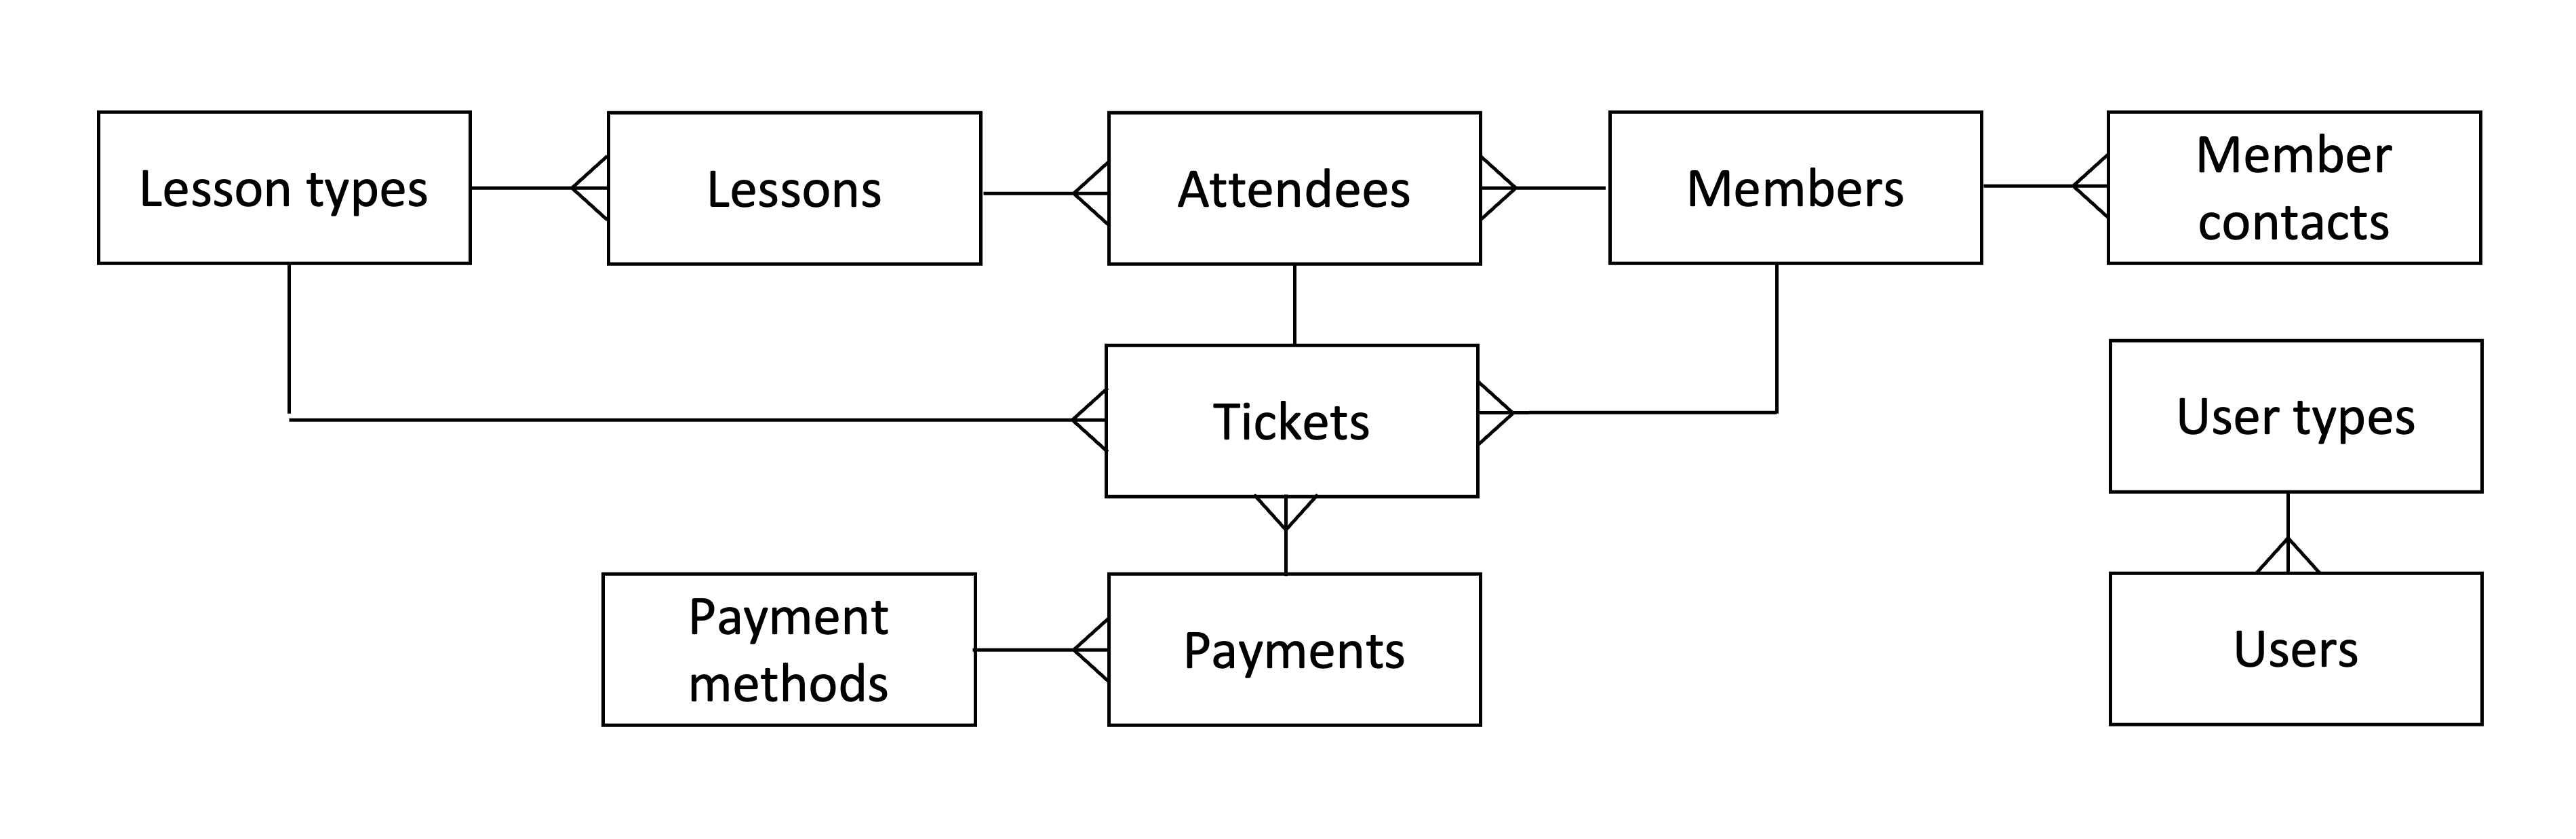
\includegraphics[width=\linewidth]{erd.png}}
    \caption{Entity relationship diagram showing the planned database table structure}
    \label{fig:erd}
\end{figure}

PostgreSQL was chosen as the relational database for this project. It is licensed under the Postgresql license, permitting use without cost or requiring written consent. Alternatives were considered, including MySQL and non-relational databases such as MongoDB; however, Postgres' performance with small and large datasets and supporting tables with relationships proved the best option for this project \parencite{arctype_performance_2021}.

Postgres also provides internal functionality for data interaction through functions called triggers. These can be activated on the change of a record and perform additional queries, including the addition, modification and deletion of records. The original intention was to use these triggers on views to prevent direct access to tables and employ the Command Query Responsibility Segregation (CQRS) pattern for payments and purchases. This design pattern segregates reads from writes, allowing greater flexibility, performance, and scalability. However, utilising this would clash with the SOLID design principle outlined at the beginning of this section, as the database would no longer only handle data storage but also perform calculations. For this reason, CQRS and event sourcing were dropped from the implementation in favour of direct table access.


%----------------------------------------------------------------------------------------
%	4. API design
%----------------------------------------------------------------------------------------

\section{API design}
The logical layer is responsible for the interaction and processing between the presentation layer's requests and the data layer's storage and retrieval in the database.

The user stories provide a flow which starts with a user interaction within the interface, triggering operations to achieve its task. Breaking down the processes within each user story revealed the operations the API would need to support to achieve each desired outcome.

Before development, the online tool OpenAPI within its online editor Swagger was used to create documentation to follow during development. It was later used to test each endpoint provided the correct response based on outlined behaviour of the documentation.

\begin{figure}[ht!]
    \centerline{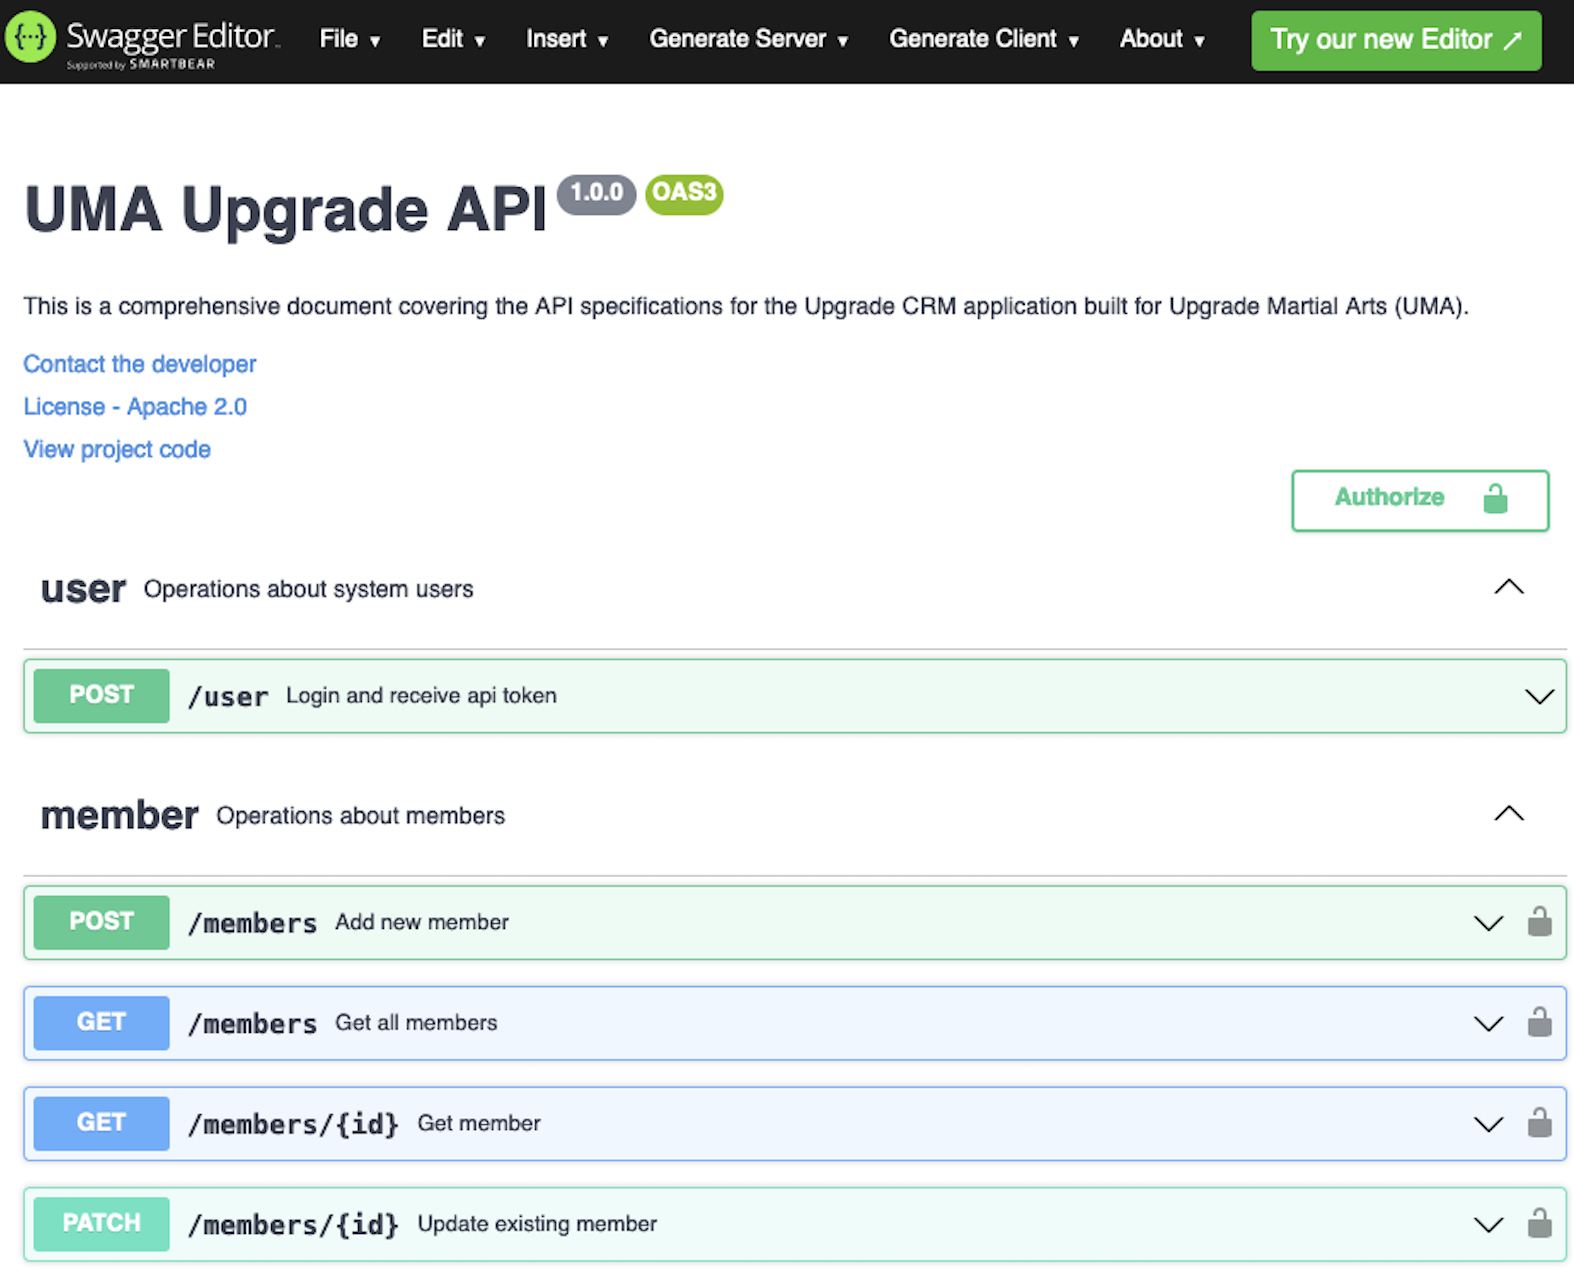
\includegraphics[width=\linewidth]{swagger.png}}
    \caption{Swagger editor showing API routes available}
    \label{fig:swagger}
\end{figure}

The MVC pattern was used in the design of the API architecture. Much like the 3-tier architecture used at the system level, the MVC design pattern also uses three layers: the model, the view and the controller.

In the context of an API, the model represents the retrieval and storage of the state within the database. These interactions could use single SQL queries to perform CRUD operations: create, read, update and delete.

The view is responsible for interaction with the logic layer and is represented as endpoints in which other software could make requests and receive responses.

The controller ties together the API endpoint and database interaction, allowing more complex operations to occur. This includes handling input validation, verifying access permissions and providing the correct error codes and responses, which were utilised heavily in each endpoint.

\begin{figure}[ht!]
    \centerline{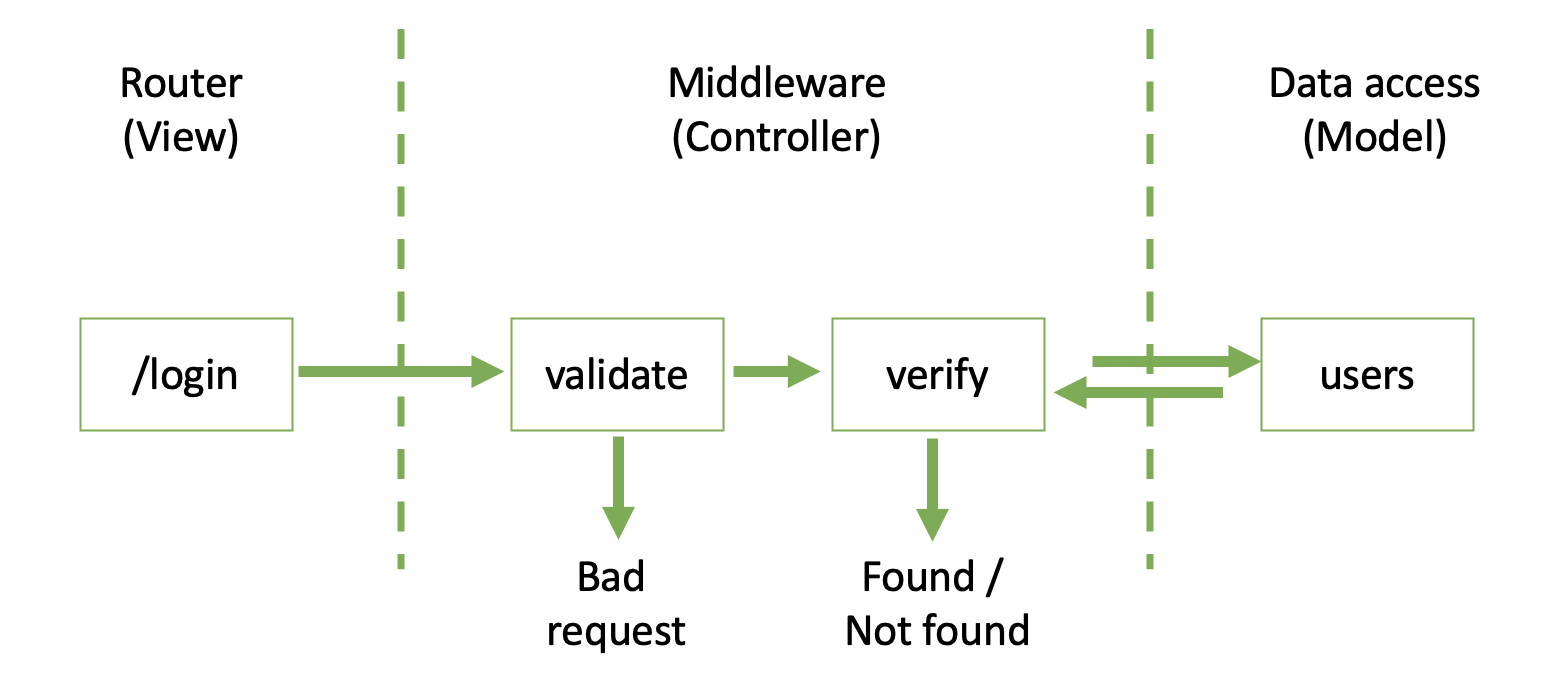
\includegraphics[width=\linewidth]{api-architecture.png}}
    \caption{API design architecture example using login route}
    \label{fig:apiarc}
\end{figure}

A flat endpoint style was implemented to simplify the interaction between the UI and API, making for an uncomplicated URL hierarchy and standardising future additions. This was further combined with standard JSON object layouts that could be easily handled and parsed at both ends.

NodeJS was selected with two main packages to interface with the presentation and data layers. The express package provided the ability to handle incoming requests and responses in a structured way. In addition, its routers provided a tidy method of segregating the launcher from each endpoint's functionality as the view. The PG package provided an interface for SQL queries on a database. These exist within service files and represent the model section of this design.

%----------------------------------------------------------------------------------------
%	5. User interface design
%----------------------------------------------------------------------------------------

\section{User interface design}

The presentation layer facilitates user interaction through inputs and visual displays representing the data. The requirements outlined the need for access across many devices. With the extreme size differences, designs for mobile and desktop views were created.

Shared components such as navigation bars, card views for summary data and common form elements, including buttons, text boxes and drop-down menus, were carefully designed. Next, the logo and colour schemes were added to these elements, where a general theme emerged and a style was established. These components were tied together into full-page designs as wireframes. These were designed to fit the user story interactions detailed in the requirements.

React selected with its component design principle. Reusable components will make a comprehensive application easier to manage. The same language as the API makes hand-off to another developer far more manageable than if the system used two different languages.

\subsection{User experience}
Great care was taken with considerations for the user experience (UX). Good UX creates a positive experience for the users of the system \parencite{yablonski_home_nodate} and makes for easier and as a result faster operation of the system.

\subsection{Wireframes}

\begin{figure}[ht!]
    \centerline{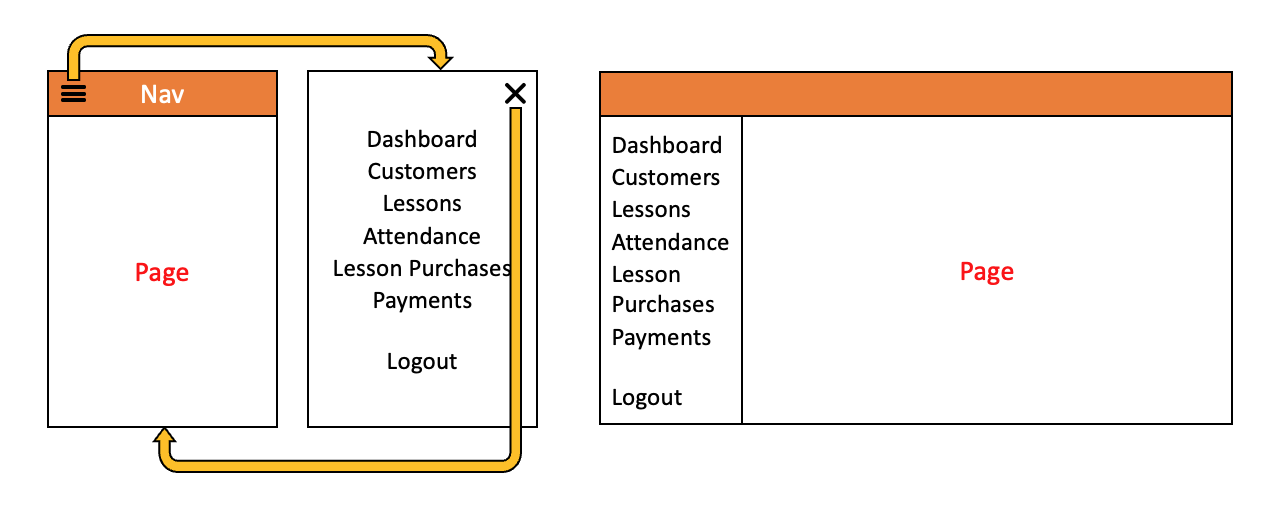
\includegraphics[width=\linewidth]{nav-wireframe.png}}
    \caption{Navigation wireframe design for mobile (left) and desktop (right)}
    \label{fig:navwireframe}
\end{figure}

\begin{figure}[ht!]
    \centerline{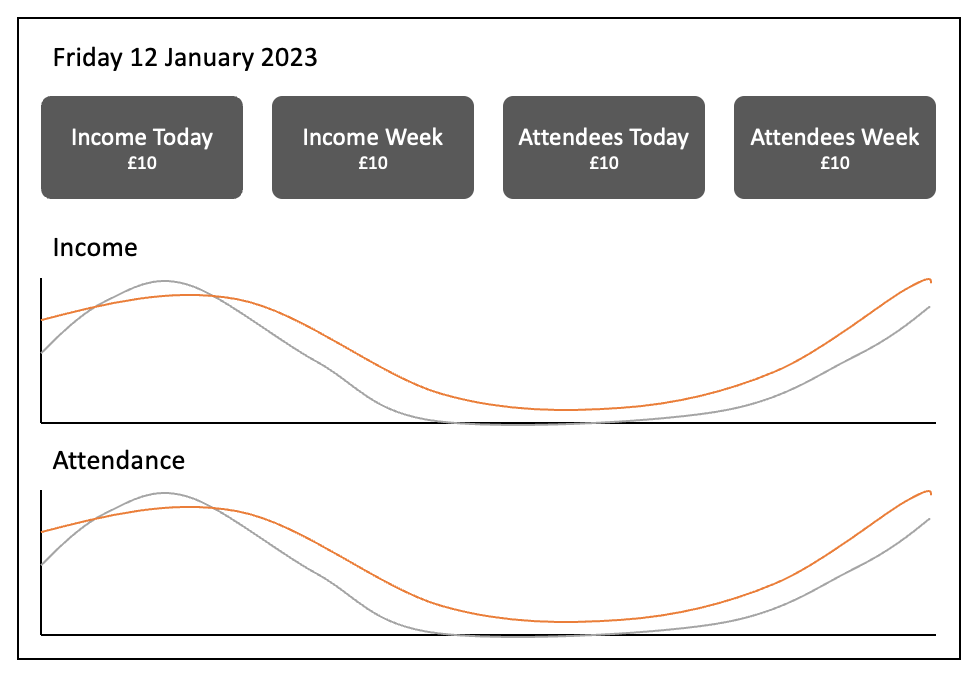
\includegraphics[width=\linewidth]{dashboard-wireframe.png}}
    \caption{Dashboard wireframe design}
    \label{fig:dashwire}
\end{figure}

\begin{figure}[ht!]
    \centerline{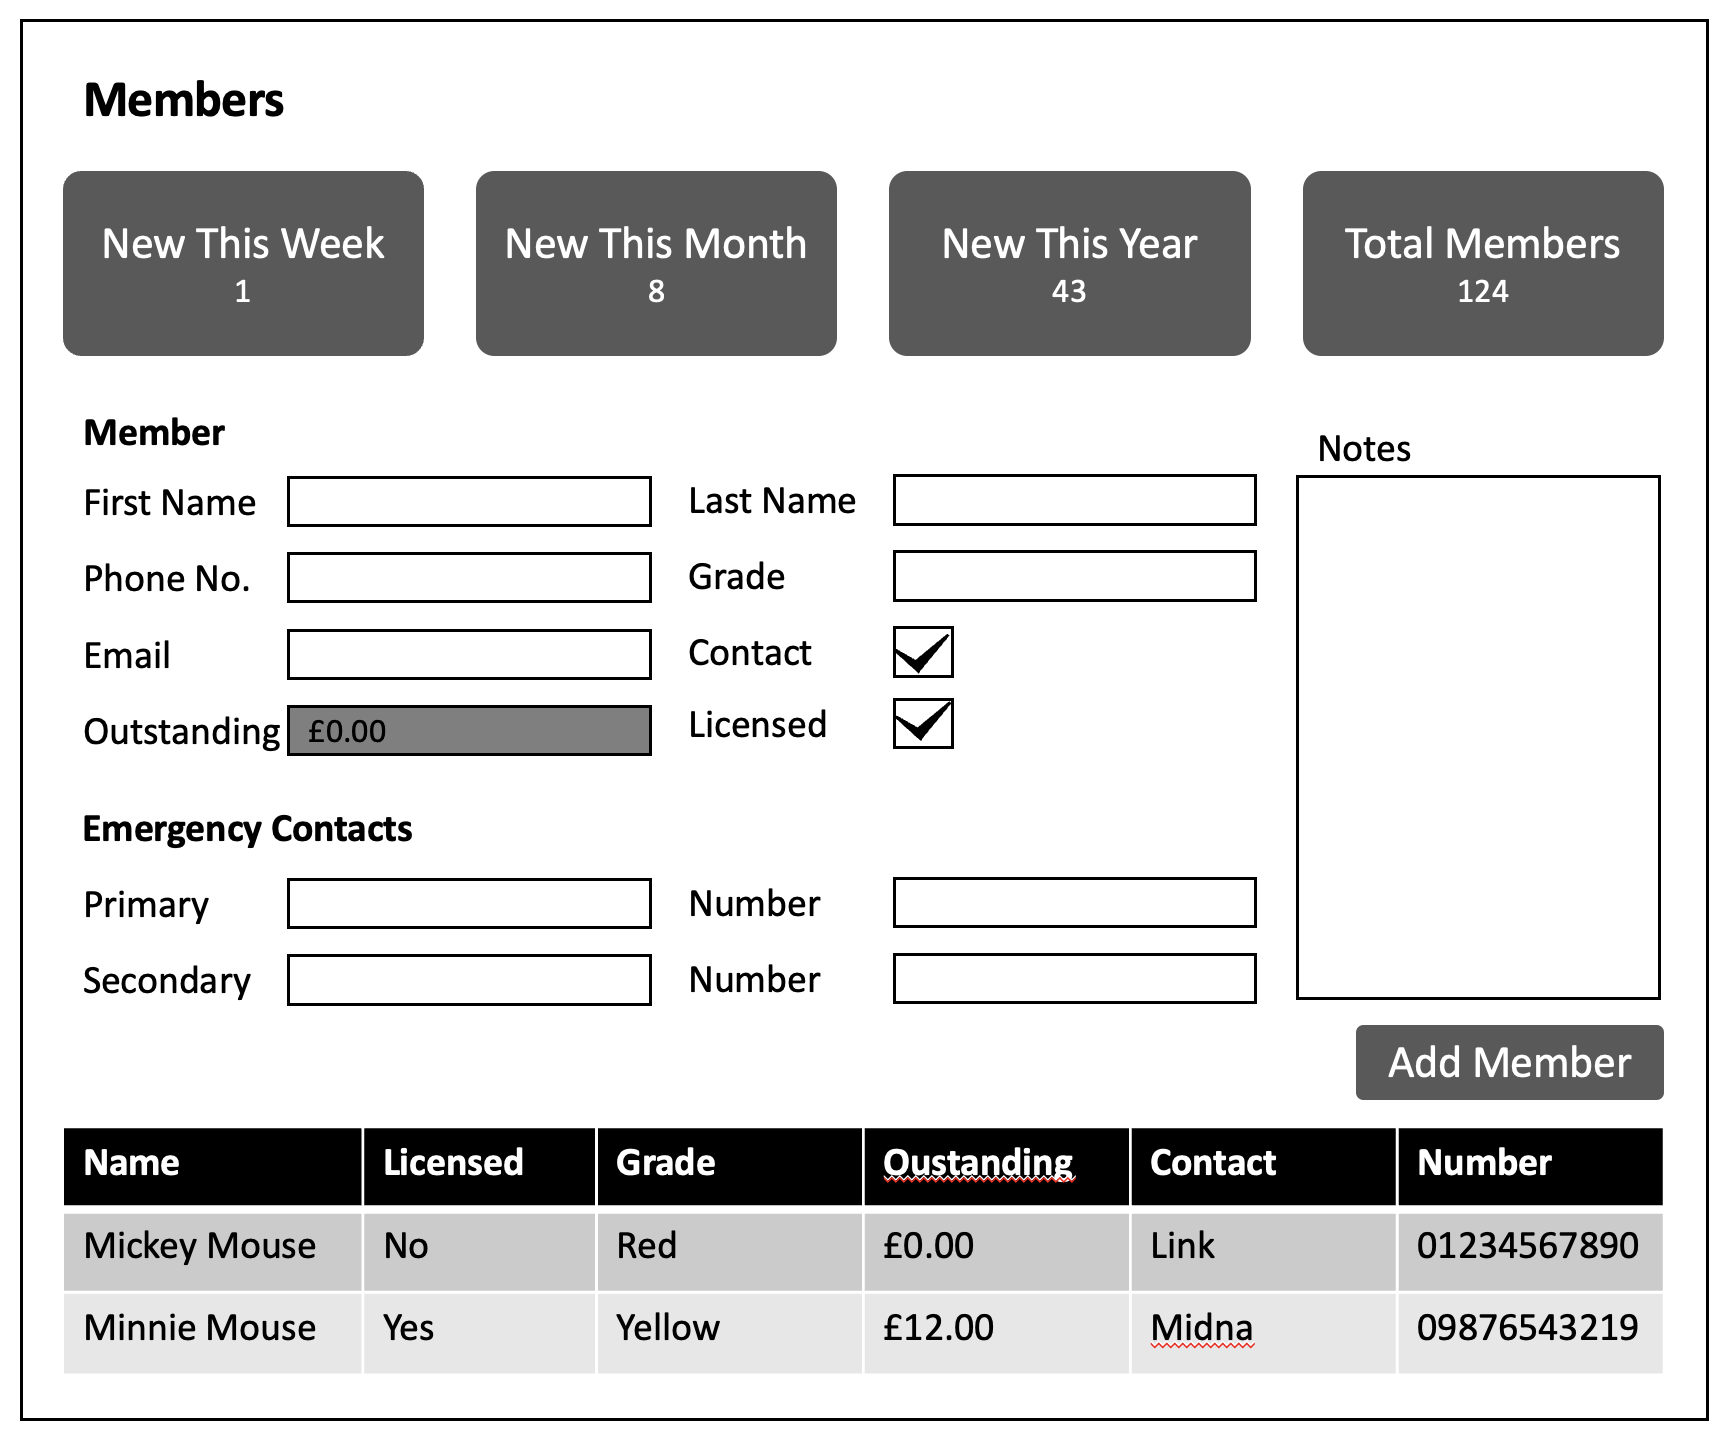
\includegraphics[width=\linewidth]{wireframe-members.png}}
    \caption{Members wireframe design}
    \label{fig:wiremembers}
\end{figure}

\begin{figure}[ht!]
    \centerline{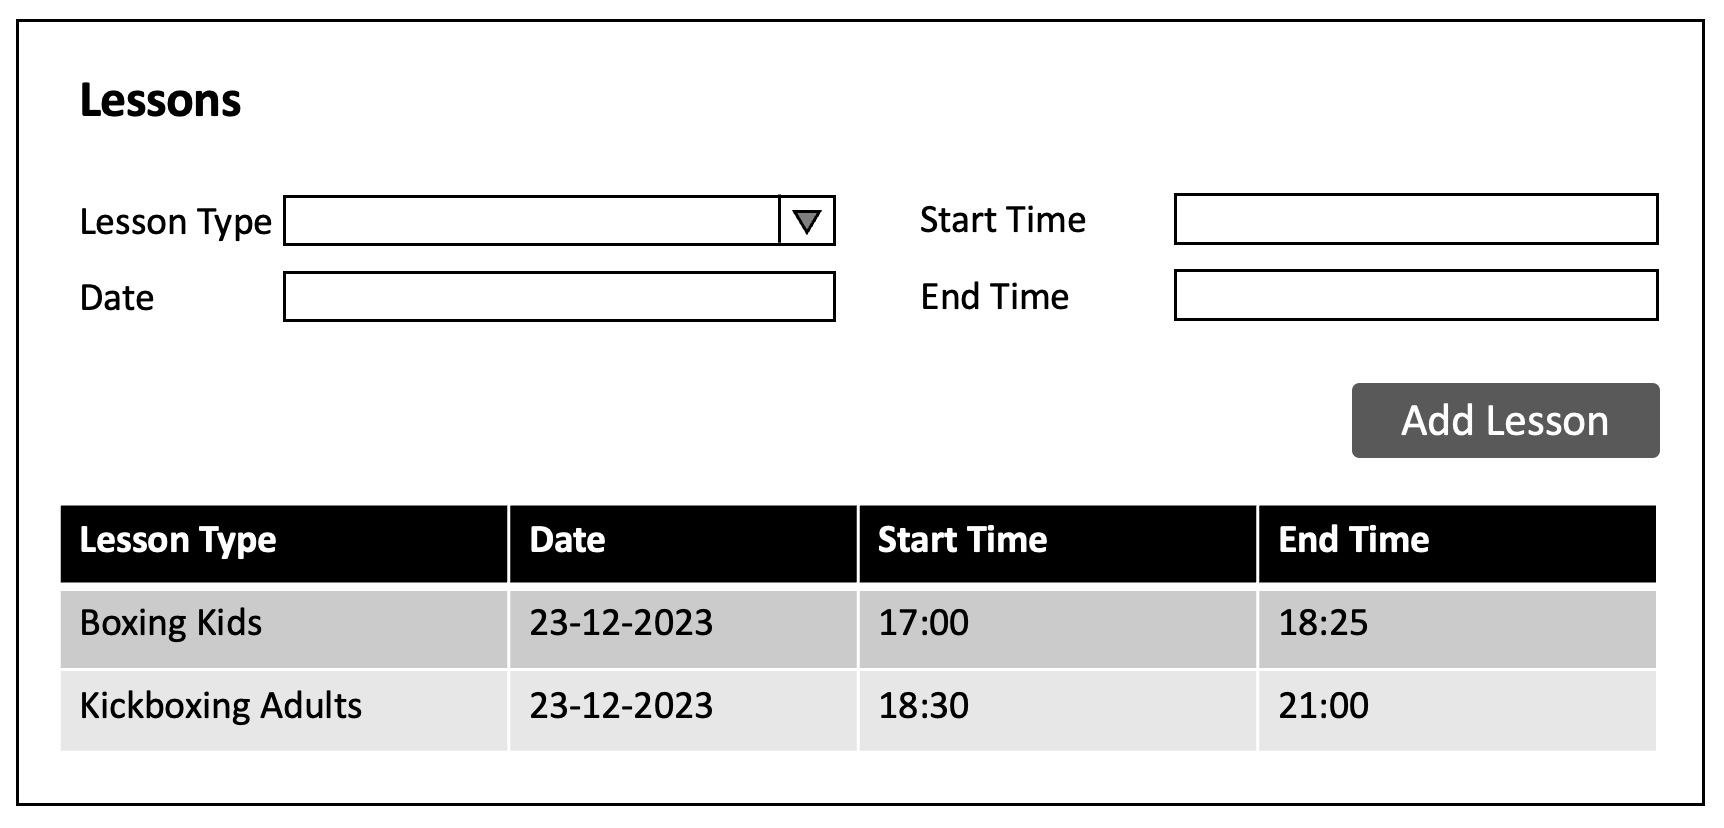
\includegraphics[width=\linewidth]{wireframe-lessons.png}}
    \caption{Lessons wireframe design}
    \label{fig:wirelessons}
\end{figure}

\begin{figure}[ht!]
    \centerline{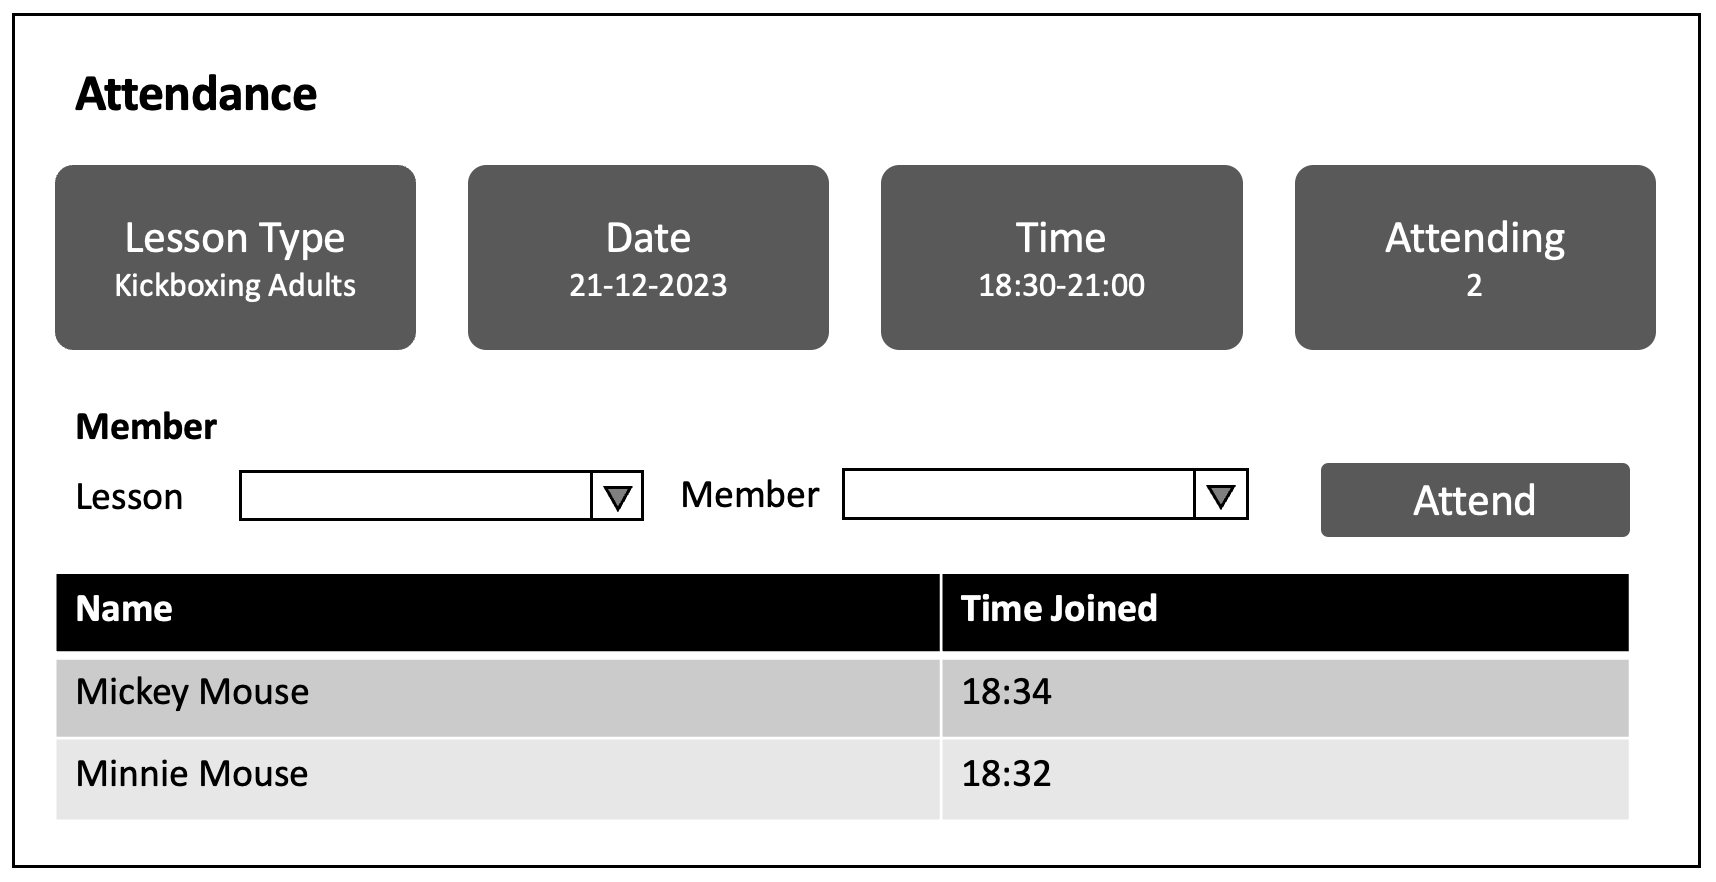
\includegraphics[width=\linewidth]{wireframe-attendances.png}}
    \caption{Attendances wireframe design}
    \label{fig:wireattendance}
\end{figure}

\begin{figure}[ht!]
    \centerline{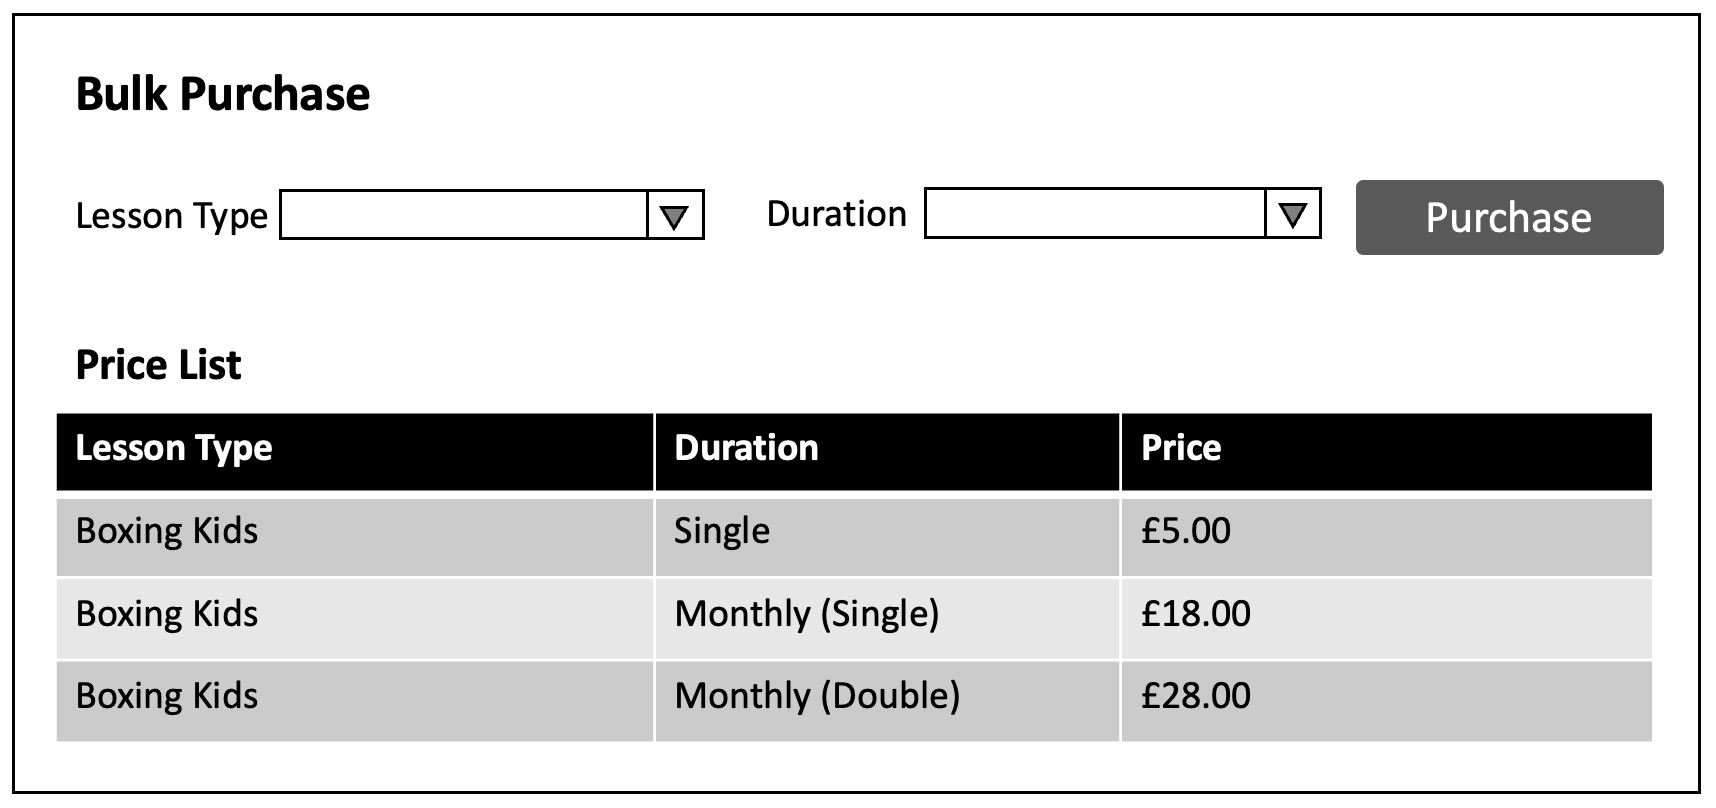
\includegraphics[width=\linewidth]{wireframe-bulk-purchase.png}}
    \caption{Purchases wireframe design}
    \label{fig:wirepurchase}
\end{figure}

\begin{figure}[ht!]
    \centerline{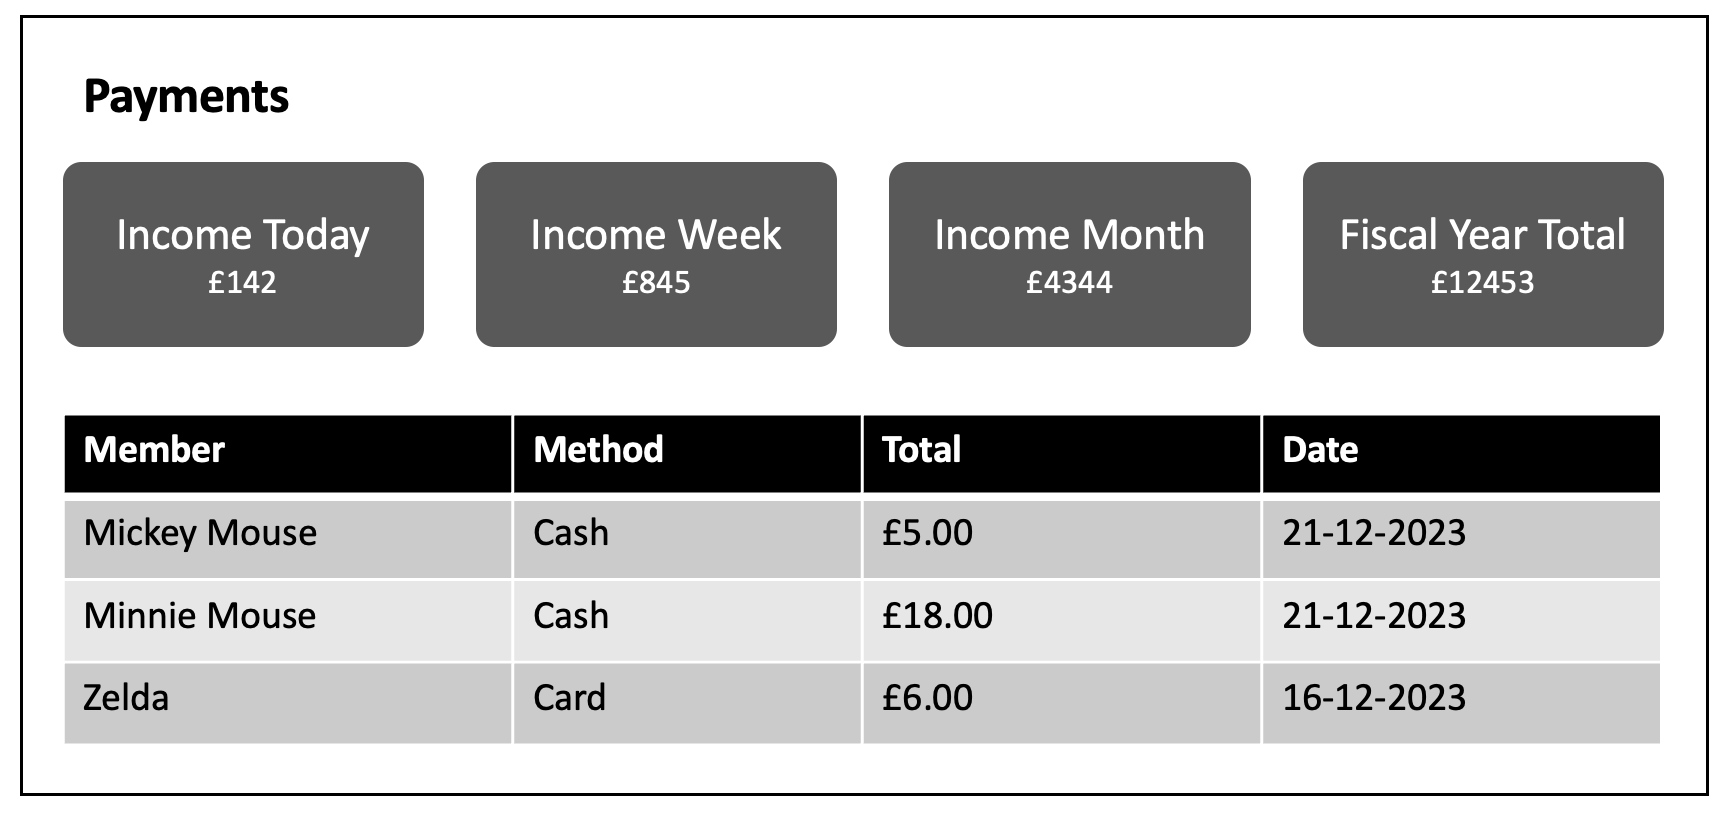
\includegraphics[width=\linewidth]{wireframe-payment.png}}
    \caption{Payments wireframe design}
    \label{fig:wirepayments}
\end{figure}

%----------------------------------------------------------------------------------------
%	6. System deployment
%----------------------------------------------------------------------------------------

% \section{System deployment}

% Todo
